\originalchapter{8.06 作业7：规范、Landau几何与慢变自旋}
来源为Spring 2018 Assignment 7, 2018年4月13日发布, Barton Zwiebach. 本篇第1--7题中文转述, 解答为\textbf{AI独立解答}. 电磁式依原题Gaussian单位, $\omega_c=qB/(mc)$, 若写磁长度$\ell_B=\sqrt{\hbar c/(qB)}$则假定$qB>0$; 通用正磁长度使用$|qB|$. 第5题沿用Griffiths例题并提其Fig.10.10, 原PDF没有附书图. 此处依MIT完整圆环模型独立画能谱并推导.
\originalsection{第1题：规范协变的边界}
\begin{exercise}
$U=\e^{\ii q\Lambda/(\hbar c)}$, $\psi'=U\psi$, $A'=A+\nabla\Lambda$, $\phi'=\phi-\dot\Lambda/c$. (a)证明Schrödinger方程规范不变. (b)证明协变量$O'=UOU^{-1}$均值不变, 判和、积、位置、正则动量、速度和Hamilton算符是否协变, 后者有何限制?
\end{exercise}
\begin{solution}
$\Pi=p-qA/c$, 直接微分$\Pi' U\psi=U\Pi\psi$. 因$i\hbar\partial_t(U\psi)=U(i\hbar\dot\psi)-q\dot\Lambda U\psi/c$, 新Hamilton算符$H'=UH U^{-1}-q\dot\Lambda/c$使等式成立. 协变均值$\bra{U\psi}(UOU^{-1})\ket{U\psi}=\bra\psi O\ket\psi$, $U$幺正.

协变量的和、积保持协变, 但积未必Hermitian, 因而不必仍可作观测量. 位置乘法与$U$对易且形式不变, 协变. 正则$p$的规定形式仍$-\ii\hbar\nabla$, 但$UpU^{-1}=p-q\nabla\Lambda/c$, 不协变; 速度$\Pi/m$协变. $H$任意含时规范下多$-q\dot\Lambda/c$, 一般不协变. 当$\dot\Lambda=0$时才严格$H'=UHU^{-1}$; 空间常但含时的$\dot\Lambda$使整体能量零点随时变, 仍不满足严格定义. 能量数值本身依标势规范, 动力学与物理结果保持不变.
\end{solution}
\originalsection{第2题：经典圆轨道中心}
\begin{exercise}
均匀$B\hat z$、二维运动, 由Lorentz力解轨道, 求中心$X=x+v_y/\omega_c,Y=y-v_x/\omega_c$并证守恒.
\end{exercise}
\begin{solution}
$\dot v_x=\omega_cv_y,\dot v_y=-\omega_cv_x$. 可写$x=X+R\cos(\omega_ct+\varphi)$,$y=Y-R\sin(\omega_ct+\varphi)$, 两导数代回力式, $R\ge0$, $\omega_c$带电荷方向符号. 由轨道得给定两中心表达, 亦直接$\dot X=v_x+\dot v_y/\omega_c=0$, $\dot Y=v_y-\dot v_x/\omega_c=0$. 轨道方向取决$qB$符号, 角速率绝对值$|\omega_c|$.
\end{solution}
\originalsection{第3题：不选规范的量子轨道}
\begin{exercise}
(a)任意磁场求$[v_x,v_y]$. 常$B$时(b)(c)求中心$X,Y$协变性、对易子与守恒. (d)(e)求$R^2=X^2+Y^2$及$r_c^2=(x-X)^2+(y-Y)^2$谱. (f)构造在圆规范变成正则$L_z$的协变角动量, 表成两半径平方差.
\end{exercise}
\begin{solution}
$[\Pi_x,\Pi_y]=\ii\hbar q(\partial_xA_y-\partial_yA_x)/c$, 所以$[v_x,v_y]=\ii\hbar qB_z(x)/(m^2c)$. 常场中心是位置加协变速度, 同样协变. 逐项对易$[X,Y]=-\ii\hbar/(m\omega_c)=-\ii\ell_B^2$（$qB>0$）, $[X,v_x]=[X,v_y]=[Y,v_x]=[Y,v_y]=0$. 因$H=m(v_x^2+v_y^2)/2$, $X,Y$均守恒而不能同时有确定值.

定义$b=(X-\ii Y)/(\sqrt2\ell_B)$, $[b,b^\dagger]=1$, 故$R^2=\ell_B^2(2b^\dagger b+1)$, 谱$(2n_g+1)\ell_B^2$. 独立回旋坐标$\eta_x=x-X=-v_y/\omega_c,\eta_y=y-Y=v_x/\omega_c$, 对易$[\eta_x,\eta_y]=+\ii\ell_B^2$, 所以$r_c^2$谱$(2n_c+1)\ell_B^2$. 两种振子自由度对易, 第一标轨道中心简并, 第二标Landau能量$H=m\omega_c^2r_c^2/2=\hbar\omega_c(n_c+1/2)$.

要求圆规范$A=B(-y,x)/2$还原$x p_y-y p_x$, 得$\mathcal L_z=m(xv_y-yv_x)+qB(x^2+y^2)/(2c)$. 两项都协变; 展开中心平方得$\mathcal L_z=m\omega_c(R^2-r_c^2)/2$, 因而守恒. 对$qB<0$相应谱尺度用$|\omega_c|$, 对易与角动量有向符号保留.
\end{solution}
\originalsection{第4题：带场的电流密度}
\begin{exercise}
从最小耦合方程求概率流$J=\hbar\operatorname{Im}(\psi^*\nabla\psi)/m-q|\psi|^2A/(mc)$, 核$j=qJ$单位与规范不变性.
\end{exercise}
\begin{solution}
先展开$\Pi^2\psi=-\hbar^2\nabla^2\psi+(\ii\hbar q/c)[(\nabla\cdot A)\psi+2A\cdot\nabla\psi]+q^2A^2\psi/c^2$. 将$H\psi$与共轭相乘相减, 标势项消去, 展开$\Pi^2$的交叉梯度成为$-\nabla\cdot[-qA|\psi|^2/(mc)]$, 自由二阶导给原概率流散度. 所以$\partial_t|\psi|^2+\nabla\cdot J=0$, $J=\operatorname{Re}(\psi^*v\psi)$是位置时间函数, 不是算符. 三维$J$单位$L^{-2}T^{-1}$, 乘电荷为单位面积单位时间电荷, 即电流密度. 变换后$\psi'^*\nabla\psi'=\psi^*\nabla\psi+\ii q|\psi|^2\nabla\Lambda/(\hbar c)$, 虚部新增项与$A'$新增项恰抵消, 所以$J'=J$.
\end{solution}
\originalsection{第5题：环绕磁通的Aharonov--Bohm谱}
\begin{exercise}
半径$a$的无限长螺线管内部场$B_0\hat z$, 外部0. 带电粒子只在外部半径$b>a$圆环运动. (a)求柱对称矢势. (b)(c)写Hamilton算符、本征态和能量. (d)改变磁通有何谱周期? (e)为何局域外部态可以消去矢势, 整环延展态却一般不行?
\end{exercise}
\begin{solution}
取$A_\phi=B_0r/2$于管内, $A_\phi=B_0a^2/(2r)=\Phi/(2\pi r)$于管外, $\Phi=\pi a^2B_0$. 直接$\frac1r\partial_r(rA_\phi)$给分段磁场, 环路积分给磁通. 在环上
\[
H=\frac{\hbar^2}{2mb^2}(-\ii\partial_\phi-\eta)^2,\quad
\eta=\frac{q\Phi}{2\pi\hbar c},\quad
\psi_n=\frac{\e^{\ii n\phi}}{\sqrt{2\pi}},\quad
E_n=\frac{\hbar^2(n-\eta)^2}{2mb^2}.
\]
周期边界使$n\in\mathbb Z$. $\eta\to\eta+1$可由$n\to n+1$重排, 所以整个谱以$\Phi_0=hc/|q|$周期. 整数通量$\Phi=m\Phi_0$时全谱与零通量一致, 因而谱只保留模$\Phi_0$的通量信息. 固定$n$分支是抛物线而不周期, 谱还对$\eta\to-\eta$相同; 单凭谱不能区分磁通方向.

在不绕一整圈的局部角区间, $\Lambda=-\Phi\phi/(2\pi)$使$A+\nabla\Lambda=0$. 全环规范相位为$\e^{-\ii\eta\phi}$, 绕一圈多$\e^{-2\pi\ii\eta}$, 除整数$\eta$不能保持单值态. 局域缺陷势也是同一局部幺正共轭下的乘法势, 在不绕环的理想支撑近似中, 困陷态能量与无螺线管时相同. 因而局部消场不消除整环的通量相位. 原件未附书图; 以下为本册算式产生的能谱.
\begin{center}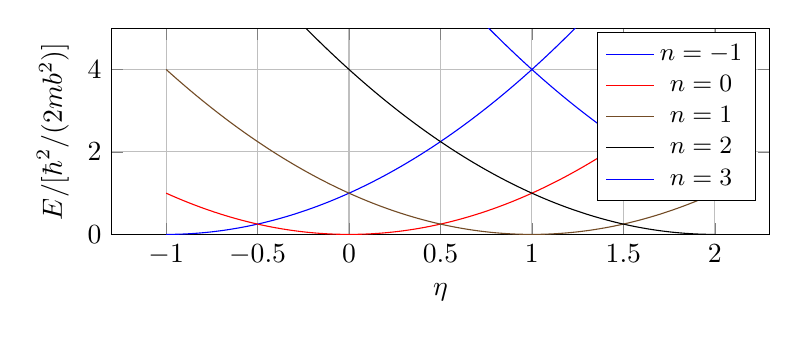
\begin{tikzpicture}
\begin{axis}[width=.82\textwidth,height=4.2cm,xlabel={$\eta$},ylabel={$E/[\hbar^2/(2mb^2)]$},grid=major,legend style={font=\small},ymin=0,ymax=5]
\addplot+[mark=none] coordinates{(-1,0) (-0.983333333,0.000277777778) (-0.966666667,0.00111111111) (-0.95,0.0025) (-0.933333333,0.00444444444) (-0.916666667,0.00694444444) (-0.9,0.01) (-0.883333333,0.0136111111) (-0.866666667,0.0177777778) (-0.85,0.0225) (-0.833333333,0.0277777778) (-0.816666667,0.0336111111) (-0.8,0.04) (-0.783333333,0.0469444444) (-0.766666667,0.0544444444) (-0.75,0.0625) (-0.733333333,0.0711111111) (-0.716666667,0.0802777778) (-0.7,0.09) (-0.683333333,0.100277778) (-0.666666667,0.111111111) (-0.65,0.1225) (-0.633333333,0.134444444) (-0.616666667,0.146944444) (-0.6,0.16) (-0.583333333,0.173611111) (-0.566666667,0.187777778) (-0.55,0.2025) (-0.533333333,0.217777778) (-0.516666667,0.233611111) (-0.5,0.25) (-0.483333333,0.266944444) (-0.466666667,0.284444444) (-0.45,0.3025) (-0.433333333,0.321111111) (-0.416666667,0.340277778) (-0.4,0.36) (-0.383333333,0.380277778) (-0.366666667,0.401111111) (-0.35,0.4225) (-0.333333333,0.444444444) (-0.316666667,0.466944444) (-0.3,0.49) (-0.283333333,0.513611111) (-0.266666667,0.537777778) (-0.25,0.5625) (-0.233333333,0.587777778) (-0.216666667,0.613611111) (-0.2,0.64) (-0.183333333,0.666944444) (-0.166666667,0.694444444) (-0.15,0.7225) (-0.133333333,0.751111111) (-0.116666667,0.780277778) (-0.1,0.81) (-0.0833333333,0.840277778) (-0.0666666667,0.871111111) (-0.05,0.9025) (-0.0333333333,0.934444444) (-0.0166666667,0.966944444) (0,1) (0.0166666667,1.03361111) (0.0333333333,1.06777778) (0.05,1.1025) (0.0666666667,1.13777778) (0.0833333333,1.17361111) (0.1,1.21) (0.116666667,1.24694444) (0.133333333,1.28444444) (0.15,1.3225) (0.166666667,1.36111111) (0.183333333,1.40027778) (0.2,1.44) (0.216666667,1.48027778) (0.233333333,1.52111111) (0.25,1.5625) (0.266666667,1.60444444) (0.283333333,1.64694444) (0.3,1.69) (0.316666667,1.73361111) (0.333333333,1.77777778) (0.35,1.8225) (0.366666667,1.86777778) (0.383333333,1.91361111) (0.4,1.96) (0.416666667,2.00694444) (0.433333333,2.05444444) (0.45,2.1025) (0.466666667,2.15111111) (0.483333333,2.20027778) (0.5,2.25) (0.516666667,2.30027778) (0.533333333,2.35111111) (0.55,2.4025) (0.566666667,2.45444444) (0.583333333,2.50694444) (0.6,2.56) (0.616666667,2.61361111) (0.633333333,2.66777778) (0.65,2.7225) (0.666666667,2.77777778) (0.683333333,2.83361111) (0.7,2.89) (0.716666667,2.94694444) (0.733333333,3.00444444) (0.75,3.0625) (0.766666667,3.12111111) (0.783333333,3.18027778) (0.8,3.24) (0.816666667,3.30027778) (0.833333333,3.36111111) (0.85,3.4225) (0.866666667,3.48444444) (0.883333333,3.54694444) (0.9,3.61) (0.916666667,3.67361111) (0.933333333,3.73777778) (0.95,3.8025) (0.966666667,3.86777778) (0.983333333,3.93361111) (1,4) (1.01666667,4.06694444) (1.03333333,4.13444444) (1.05,4.2025) (1.06666667,4.27111111) (1.08333333,4.34027778) (1.1,4.41) (1.11666667,4.48027778) (1.13333333,4.55111111) (1.15,4.6225) (1.16666667,4.69444444) (1.18333333,4.76694444) (1.2,4.84) (1.21666667,4.91361111) (1.23333333,4.98777778) (1.25,5.0625) (1.26666667,5.13777778) (1.28333333,5.21361111) (1.3,5.29) (1.31666667,5.36694444) (1.33333333,5.44444444) (1.35,5.5225) (1.36666667,5.60111111) (1.38333333,5.68027778) (1.4,5.76) (1.41666667,5.84027778) (1.43333333,5.92111111) (1.45,6.0025) (1.46666667,6.08444444) (1.48333333,6.16694444) (1.5,6.25) (1.51666667,6.33361111) (1.53333333,6.41777778) (1.55,6.5025) (1.56666667,6.58777778) (1.58333333,6.67361111) (1.6,6.76) (1.61666667,6.84694444) (1.63333333,6.93444444) (1.65,7.0225) (1.66666667,7.11111111) (1.68333333,7.20027778) (1.7,7.29) (1.71666667,7.38027778) (1.73333333,7.47111111) (1.75,7.5625) (1.76666667,7.65444444) (1.78333333,7.74694444) (1.8,7.84) (1.81666667,7.93361111) (1.83333333,8.02777778) (1.85,8.1225) (1.86666667,8.21777778) (1.88333333,8.31361111) (1.9,8.41) (1.91666667,8.50694444) (1.93333333,8.60444444) (1.95,8.7025) (1.96666667,8.80111111) (1.98333333,8.90027778) (2,9)};
\addlegendentry{$n=-1$}
\addplot+[mark=none] coordinates{(-1,1) (-0.983333333,0.966944444) (-0.966666667,0.934444444) (-0.95,0.9025) (-0.933333333,0.871111111) (-0.916666667,0.840277778) (-0.9,0.81) (-0.883333333,0.780277778) (-0.866666667,0.751111111) (-0.85,0.7225) (-0.833333333,0.694444444) (-0.816666667,0.666944444) (-0.8,0.64) (-0.783333333,0.613611111) (-0.766666667,0.587777778) (-0.75,0.5625) (-0.733333333,0.537777778) (-0.716666667,0.513611111) (-0.7,0.49) (-0.683333333,0.466944444) (-0.666666667,0.444444444) (-0.65,0.4225) (-0.633333333,0.401111111) (-0.616666667,0.380277778) (-0.6,0.36) (-0.583333333,0.340277778) (-0.566666667,0.321111111) (-0.55,0.3025) (-0.533333333,0.284444444) (-0.516666667,0.266944444) (-0.5,0.25) (-0.483333333,0.233611111) (-0.466666667,0.217777778) (-0.45,0.2025) (-0.433333333,0.187777778) (-0.416666667,0.173611111) (-0.4,0.16) (-0.383333333,0.146944444) (-0.366666667,0.134444444) (-0.35,0.1225) (-0.333333333,0.111111111) (-0.316666667,0.100277778) (-0.3,0.09) (-0.283333333,0.0802777778) (-0.266666667,0.0711111111) (-0.25,0.0625) (-0.233333333,0.0544444444) (-0.216666667,0.0469444444) (-0.2,0.04) (-0.183333333,0.0336111111) (-0.166666667,0.0277777778) (-0.15,0.0225) (-0.133333333,0.0177777778) (-0.116666667,0.0136111111) (-0.1,0.01) (-0.0833333333,0.00694444444) (-0.0666666667,0.00444444444) (-0.05,0.0025) (-0.0333333333,0.00111111111) (-0.0166666667,0.000277777778) (0,0) (0.0166666667,0.000277777778) (0.0333333333,0.00111111111) (0.05,0.0025) (0.0666666667,0.00444444444) (0.0833333333,0.00694444444) (0.1,0.01) (0.116666667,0.0136111111) (0.133333333,0.0177777778) (0.15,0.0225) (0.166666667,0.0277777778) (0.183333333,0.0336111111) (0.2,0.04) (0.216666667,0.0469444444) (0.233333333,0.0544444444) (0.25,0.0625) (0.266666667,0.0711111111) (0.283333333,0.0802777778) (0.3,0.09) (0.316666667,0.100277778) (0.333333333,0.111111111) (0.35,0.1225) (0.366666667,0.134444444) (0.383333333,0.146944444) (0.4,0.16) (0.416666667,0.173611111) (0.433333333,0.187777778) (0.45,0.2025) (0.466666667,0.217777778) (0.483333333,0.233611111) (0.5,0.25) (0.516666667,0.266944444) (0.533333333,0.284444444) (0.55,0.3025) (0.566666667,0.321111111) (0.583333333,0.340277778) (0.6,0.36) (0.616666667,0.380277778) (0.633333333,0.401111111) (0.65,0.4225) (0.666666667,0.444444444) (0.683333333,0.466944444) (0.7,0.49) (0.716666667,0.513611111) (0.733333333,0.537777778) (0.75,0.5625) (0.766666667,0.587777778) (0.783333333,0.613611111) (0.8,0.64) (0.816666667,0.666944444) (0.833333333,0.694444444) (0.85,0.7225) (0.866666667,0.751111111) (0.883333333,0.780277778) (0.9,0.81) (0.916666667,0.840277778) (0.933333333,0.871111111) (0.95,0.9025) (0.966666667,0.934444444) (0.983333333,0.966944444) (1,1) (1.01666667,1.03361111) (1.03333333,1.06777778) (1.05,1.1025) (1.06666667,1.13777778) (1.08333333,1.17361111) (1.1,1.21) (1.11666667,1.24694444) (1.13333333,1.28444444) (1.15,1.3225) (1.16666667,1.36111111) (1.18333333,1.40027778) (1.2,1.44) (1.21666667,1.48027778) (1.23333333,1.52111111) (1.25,1.5625) (1.26666667,1.60444444) (1.28333333,1.64694444) (1.3,1.69) (1.31666667,1.73361111) (1.33333333,1.77777778) (1.35,1.8225) (1.36666667,1.86777778) (1.38333333,1.91361111) (1.4,1.96) (1.41666667,2.00694444) (1.43333333,2.05444444) (1.45,2.1025) (1.46666667,2.15111111) (1.48333333,2.20027778) (1.5,2.25) (1.51666667,2.30027778) (1.53333333,2.35111111) (1.55,2.4025) (1.56666667,2.45444444) (1.58333333,2.50694444) (1.6,2.56) (1.61666667,2.61361111) (1.63333333,2.66777778) (1.65,2.7225) (1.66666667,2.77777778) (1.68333333,2.83361111) (1.7,2.89) (1.71666667,2.94694444) (1.73333333,3.00444444) (1.75,3.0625) (1.76666667,3.12111111) (1.78333333,3.18027778) (1.8,3.24) (1.81666667,3.30027778) (1.83333333,3.36111111) (1.85,3.4225) (1.86666667,3.48444444) (1.88333333,3.54694444) (1.9,3.61) (1.91666667,3.67361111) (1.93333333,3.73777778) (1.95,3.8025) (1.96666667,3.86777778) (1.98333333,3.93361111) (2,4)};
\addlegendentry{$n=0$}
\addplot+[mark=none] coordinates{(-1,4) (-0.983333333,3.93361111) (-0.966666667,3.86777778) (-0.95,3.8025) (-0.933333333,3.73777778) (-0.916666667,3.67361111) (-0.9,3.61) (-0.883333333,3.54694444) (-0.866666667,3.48444444) (-0.85,3.4225) (-0.833333333,3.36111111) (-0.816666667,3.30027778) (-0.8,3.24) (-0.783333333,3.18027778) (-0.766666667,3.12111111) (-0.75,3.0625) (-0.733333333,3.00444444) (-0.716666667,2.94694444) (-0.7,2.89) (-0.683333333,2.83361111) (-0.666666667,2.77777778) (-0.65,2.7225) (-0.633333333,2.66777778) (-0.616666667,2.61361111) (-0.6,2.56) (-0.583333333,2.50694444) (-0.566666667,2.45444444) (-0.55,2.4025) (-0.533333333,2.35111111) (-0.516666667,2.30027778) (-0.5,2.25) (-0.483333333,2.20027778) (-0.466666667,2.15111111) (-0.45,2.1025) (-0.433333333,2.05444444) (-0.416666667,2.00694444) (-0.4,1.96) (-0.383333333,1.91361111) (-0.366666667,1.86777778) (-0.35,1.8225) (-0.333333333,1.77777778) (-0.316666667,1.73361111) (-0.3,1.69) (-0.283333333,1.64694444) (-0.266666667,1.60444444) (-0.25,1.5625) (-0.233333333,1.52111111) (-0.216666667,1.48027778) (-0.2,1.44) (-0.183333333,1.40027778) (-0.166666667,1.36111111) (-0.15,1.3225) (-0.133333333,1.28444444) (-0.116666667,1.24694444) (-0.1,1.21) (-0.0833333333,1.17361111) (-0.0666666667,1.13777778) (-0.05,1.1025) (-0.0333333333,1.06777778) (-0.0166666667,1.03361111) (0,1) (0.0166666667,0.966944444) (0.0333333333,0.934444444) (0.05,0.9025) (0.0666666667,0.871111111) (0.0833333333,0.840277778) (0.1,0.81) (0.116666667,0.780277778) (0.133333333,0.751111111) (0.15,0.7225) (0.166666667,0.694444444) (0.183333333,0.666944444) (0.2,0.64) (0.216666667,0.613611111) (0.233333333,0.587777778) (0.25,0.5625) (0.266666667,0.537777778) (0.283333333,0.513611111) (0.3,0.49) (0.316666667,0.466944444) (0.333333333,0.444444444) (0.35,0.4225) (0.366666667,0.401111111) (0.383333333,0.380277778) (0.4,0.36) (0.416666667,0.340277778) (0.433333333,0.321111111) (0.45,0.3025) (0.466666667,0.284444444) (0.483333333,0.266944444) (0.5,0.25) (0.516666667,0.233611111) (0.533333333,0.217777778) (0.55,0.2025) (0.566666667,0.187777778) (0.583333333,0.173611111) (0.6,0.16) (0.616666667,0.146944444) (0.633333333,0.134444444) (0.65,0.1225) (0.666666667,0.111111111) (0.683333333,0.100277778) (0.7,0.09) (0.716666667,0.0802777778) (0.733333333,0.0711111111) (0.75,0.0625) (0.766666667,0.0544444444) (0.783333333,0.0469444444) (0.8,0.04) (0.816666667,0.0336111111) (0.833333333,0.0277777778) (0.85,0.0225) (0.866666667,0.0177777778) (0.883333333,0.0136111111) (0.9,0.01) (0.916666667,0.00694444444) (0.933333333,0.00444444444) (0.95,0.0025) (0.966666667,0.00111111111) (0.983333333,0.000277777778) (1,0) (1.01666667,0.000277777778) (1.03333333,0.00111111111) (1.05,0.0025) (1.06666667,0.00444444444) (1.08333333,0.00694444444) (1.1,0.01) (1.11666667,0.0136111111) (1.13333333,0.0177777778) (1.15,0.0225) (1.16666667,0.0277777778) (1.18333333,0.0336111111) (1.2,0.04) (1.21666667,0.0469444444) (1.23333333,0.0544444444) (1.25,0.0625) (1.26666667,0.0711111111) (1.28333333,0.0802777778) (1.3,0.09) (1.31666667,0.100277778) (1.33333333,0.111111111) (1.35,0.1225) (1.36666667,0.134444444) (1.38333333,0.146944444) (1.4,0.16) (1.41666667,0.173611111) (1.43333333,0.187777778) (1.45,0.2025) (1.46666667,0.217777778) (1.48333333,0.233611111) (1.5,0.25) (1.51666667,0.266944444) (1.53333333,0.284444444) (1.55,0.3025) (1.56666667,0.321111111) (1.58333333,0.340277778) (1.6,0.36) (1.61666667,0.380277778) (1.63333333,0.401111111) (1.65,0.4225) (1.66666667,0.444444444) (1.68333333,0.466944444) (1.7,0.49) (1.71666667,0.513611111) (1.73333333,0.537777778) (1.75,0.5625) (1.76666667,0.587777778) (1.78333333,0.613611111) (1.8,0.64) (1.81666667,0.666944444) (1.83333333,0.694444444) (1.85,0.7225) (1.86666667,0.751111111) (1.88333333,0.780277778) (1.9,0.81) (1.91666667,0.840277778) (1.93333333,0.871111111) (1.95,0.9025) (1.96666667,0.934444444) (1.98333333,0.966944444) (2,1)};
\addlegendentry{$n=1$}
\addplot+[mark=none] coordinates{(-1,9) (-0.983333333,8.90027778) (-0.966666667,8.80111111) (-0.95,8.7025) (-0.933333333,8.60444444) (-0.916666667,8.50694444) (-0.9,8.41) (-0.883333333,8.31361111) (-0.866666667,8.21777778) (-0.85,8.1225) (-0.833333333,8.02777778) (-0.816666667,7.93361111) (-0.8,7.84) (-0.783333333,7.74694444) (-0.766666667,7.65444444) (-0.75,7.5625) (-0.733333333,7.47111111) (-0.716666667,7.38027778) (-0.7,7.29) (-0.683333333,7.20027778) (-0.666666667,7.11111111) (-0.65,7.0225) (-0.633333333,6.93444444) (-0.616666667,6.84694444) (-0.6,6.76) (-0.583333333,6.67361111) (-0.566666667,6.58777778) (-0.55,6.5025) (-0.533333333,6.41777778) (-0.516666667,6.33361111) (-0.5,6.25) (-0.483333333,6.16694444) (-0.466666667,6.08444444) (-0.45,6.0025) (-0.433333333,5.92111111) (-0.416666667,5.84027778) (-0.4,5.76) (-0.383333333,5.68027778) (-0.366666667,5.60111111) (-0.35,5.5225) (-0.333333333,5.44444444) (-0.316666667,5.36694444) (-0.3,5.29) (-0.283333333,5.21361111) (-0.266666667,5.13777778) (-0.25,5.0625) (-0.233333333,4.98777778) (-0.216666667,4.91361111) (-0.2,4.84) (-0.183333333,4.76694444) (-0.166666667,4.69444444) (-0.15,4.6225) (-0.133333333,4.55111111) (-0.116666667,4.48027778) (-0.1,4.41) (-0.0833333333,4.34027778) (-0.0666666667,4.27111111) (-0.05,4.2025) (-0.0333333333,4.13444444) (-0.0166666667,4.06694444) (0,4) (0.0166666667,3.93361111) (0.0333333333,3.86777778) (0.05,3.8025) (0.0666666667,3.73777778) (0.0833333333,3.67361111) (0.1,3.61) (0.116666667,3.54694444) (0.133333333,3.48444444) (0.15,3.4225) (0.166666667,3.36111111) (0.183333333,3.30027778) (0.2,3.24) (0.216666667,3.18027778) (0.233333333,3.12111111) (0.25,3.0625) (0.266666667,3.00444444) (0.283333333,2.94694444) (0.3,2.89) (0.316666667,2.83361111) (0.333333333,2.77777778) (0.35,2.7225) (0.366666667,2.66777778) (0.383333333,2.61361111) (0.4,2.56) (0.416666667,2.50694444) (0.433333333,2.45444444) (0.45,2.4025) (0.466666667,2.35111111) (0.483333333,2.30027778) (0.5,2.25) (0.516666667,2.20027778) (0.533333333,2.15111111) (0.55,2.1025) (0.566666667,2.05444444) (0.583333333,2.00694444) (0.6,1.96) (0.616666667,1.91361111) (0.633333333,1.86777778) (0.65,1.8225) (0.666666667,1.77777778) (0.683333333,1.73361111) (0.7,1.69) (0.716666667,1.64694444) (0.733333333,1.60444444) (0.75,1.5625) (0.766666667,1.52111111) (0.783333333,1.48027778) (0.8,1.44) (0.816666667,1.40027778) (0.833333333,1.36111111) (0.85,1.3225) (0.866666667,1.28444444) (0.883333333,1.24694444) (0.9,1.21) (0.916666667,1.17361111) (0.933333333,1.13777778) (0.95,1.1025) (0.966666667,1.06777778) (0.983333333,1.03361111) (1,1) (1.01666667,0.966944444) (1.03333333,0.934444444) (1.05,0.9025) (1.06666667,0.871111111) (1.08333333,0.840277778) (1.1,0.81) (1.11666667,0.780277778) (1.13333333,0.751111111) (1.15,0.7225) (1.16666667,0.694444444) (1.18333333,0.666944444) (1.2,0.64) (1.21666667,0.613611111) (1.23333333,0.587777778) (1.25,0.5625) (1.26666667,0.537777778) (1.28333333,0.513611111) (1.3,0.49) (1.31666667,0.466944444) (1.33333333,0.444444444) (1.35,0.4225) (1.36666667,0.401111111) (1.38333333,0.380277778) (1.4,0.36) (1.41666667,0.340277778) (1.43333333,0.321111111) (1.45,0.3025) (1.46666667,0.284444444) (1.48333333,0.266944444) (1.5,0.25) (1.51666667,0.233611111) (1.53333333,0.217777778) (1.55,0.2025) (1.56666667,0.187777778) (1.58333333,0.173611111) (1.6,0.16) (1.61666667,0.146944444) (1.63333333,0.134444444) (1.65,0.1225) (1.66666667,0.111111111) (1.68333333,0.100277778) (1.7,0.09) (1.71666667,0.0802777778) (1.73333333,0.0711111111) (1.75,0.0625) (1.76666667,0.0544444444) (1.78333333,0.0469444444) (1.8,0.04) (1.81666667,0.0336111111) (1.83333333,0.0277777778) (1.85,0.0225) (1.86666667,0.0177777778) (1.88333333,0.0136111111) (1.9,0.01) (1.91666667,0.00694444444) (1.93333333,0.00444444444) (1.95,0.0025) (1.96666667,0.00111111111) (1.98333333,0.000277777778) (2,0)};
\addlegendentry{$n=2$}
\addplot+[mark=none] coordinates{(-1,16) (-0.983333333,15.8669444) (-0.966666667,15.7344444) (-0.95,15.6025) (-0.933333333,15.4711111) (-0.916666667,15.3402778) (-0.9,15.21) (-0.883333333,15.0802778) (-0.866666667,14.9511111) (-0.85,14.8225) (-0.833333333,14.6944444) (-0.816666667,14.5669444) (-0.8,14.44) (-0.783333333,14.3136111) (-0.766666667,14.1877778) (-0.75,14.0625) (-0.733333333,13.9377778) (-0.716666667,13.8136111) (-0.7,13.69) (-0.683333333,13.5669444) (-0.666666667,13.4444444) (-0.65,13.3225) (-0.633333333,13.2011111) (-0.616666667,13.0802778) (-0.6,12.96) (-0.583333333,12.8402778) (-0.566666667,12.7211111) (-0.55,12.6025) (-0.533333333,12.4844444) (-0.516666667,12.3669444) (-0.5,12.25) (-0.483333333,12.1336111) (-0.466666667,12.0177778) (-0.45,11.9025) (-0.433333333,11.7877778) (-0.416666667,11.6736111) (-0.4,11.56) (-0.383333333,11.4469444) (-0.366666667,11.3344444) (-0.35,11.2225) (-0.333333333,11.1111111) (-0.316666667,11.0002778) (-0.3,10.89) (-0.283333333,10.7802778) (-0.266666667,10.6711111) (-0.25,10.5625) (-0.233333333,10.4544444) (-0.216666667,10.3469444) (-0.2,10.24) (-0.183333333,10.1336111) (-0.166666667,10.0277778) (-0.15,9.9225) (-0.133333333,9.81777778) (-0.116666667,9.71361111) (-0.1,9.61) (-0.0833333333,9.50694444) (-0.0666666667,9.40444444) (-0.05,9.3025) (-0.0333333333,9.20111111) (-0.0166666667,9.10027778) (0,9) (0.0166666667,8.90027778) (0.0333333333,8.80111111) (0.05,8.7025) (0.0666666667,8.60444444) (0.0833333333,8.50694444) (0.1,8.41) (0.116666667,8.31361111) (0.133333333,8.21777778) (0.15,8.1225) (0.166666667,8.02777778) (0.183333333,7.93361111) (0.2,7.84) (0.216666667,7.74694444) (0.233333333,7.65444444) (0.25,7.5625) (0.266666667,7.47111111) (0.283333333,7.38027778) (0.3,7.29) (0.316666667,7.20027778) (0.333333333,7.11111111) (0.35,7.0225) (0.366666667,6.93444444) (0.383333333,6.84694444) (0.4,6.76) (0.416666667,6.67361111) (0.433333333,6.58777778) (0.45,6.5025) (0.466666667,6.41777778) (0.483333333,6.33361111) (0.5,6.25) (0.516666667,6.16694444) (0.533333333,6.08444444) (0.55,6.0025) (0.566666667,5.92111111) (0.583333333,5.84027778) (0.6,5.76) (0.616666667,5.68027778) (0.633333333,5.60111111) (0.65,5.5225) (0.666666667,5.44444444) (0.683333333,5.36694444) (0.7,5.29) (0.716666667,5.21361111) (0.733333333,5.13777778) (0.75,5.0625) (0.766666667,4.98777778) (0.783333333,4.91361111) (0.8,4.84) (0.816666667,4.76694444) (0.833333333,4.69444444) (0.85,4.6225) (0.866666667,4.55111111) (0.883333333,4.48027778) (0.9,4.41) (0.916666667,4.34027778) (0.933333333,4.27111111) (0.95,4.2025) (0.966666667,4.13444444) (0.983333333,4.06694444) (1,4) (1.01666667,3.93361111) (1.03333333,3.86777778) (1.05,3.8025) (1.06666667,3.73777778) (1.08333333,3.67361111) (1.1,3.61) (1.11666667,3.54694444) (1.13333333,3.48444444) (1.15,3.4225) (1.16666667,3.36111111) (1.18333333,3.30027778) (1.2,3.24) (1.21666667,3.18027778) (1.23333333,3.12111111) (1.25,3.0625) (1.26666667,3.00444444) (1.28333333,2.94694444) (1.3,2.89) (1.31666667,2.83361111) (1.33333333,2.77777778) (1.35,2.7225) (1.36666667,2.66777778) (1.38333333,2.61361111) (1.4,2.56) (1.41666667,2.50694444) (1.43333333,2.45444444) (1.45,2.4025) (1.46666667,2.35111111) (1.48333333,2.30027778) (1.5,2.25) (1.51666667,2.20027778) (1.53333333,2.15111111) (1.55,2.1025) (1.56666667,2.05444444) (1.58333333,2.00694444) (1.6,1.96) (1.61666667,1.91361111) (1.63333333,1.86777778) (1.65,1.8225) (1.66666667,1.77777778) (1.68333333,1.73361111) (1.7,1.69) (1.71666667,1.64694444) (1.73333333,1.60444444) (1.75,1.5625) (1.76666667,1.52111111) (1.78333333,1.48027778) (1.8,1.44) (1.81666667,1.40027778) (1.83333333,1.36111111) (1.85,1.3225) (1.86666667,1.28444444) (1.88333333,1.24694444) (1.9,1.21) (1.91666667,1.17361111) (1.93333333,1.13777778) (1.95,1.1025) (1.96666667,1.06777778) (1.98333333,1.03361111) (2,1)};
\addlegendentry{$n=3$}
\end{axis}\end{tikzpicture}\end{center}

\end{solution}
\originalsection{第6题：避免交叉与磁阱}
\begin{exercise}
自旋1/2 $H=-\mu_0\boldsymbol\sigma\cdot B(t)$,$\mu_0>0$, $B=(B_x,B_y,\gamma t)$,$\delta B=\sqrt{B_x^2+B_y^2}\ne0$, $\gamma T\gg\delta B$. (a)给保持基态的慢变条件. (b)为何近似$z-$翻到$z+$, 消去$\gamma$给$T$下界尺度. (c)质量$m$、温度$T_{\rm gas}$原子在非均匀磁阱运动, 给绝热条件. (d)解释零磁场为何危险.
\end{exercise}
\begin{solution}
两能量$\mp\mu_0|B|$, 最小隙$2\mu_0\delta B$, 转动最快在$t=0$, $|\bra-\dot H\ket+|=\mu_0\gamma$. 本册局部诊断给$\hbar\gamma/(4\mu_0\delta B^2)\ll1$, 即$\gamma\ll4\mu_0\delta B^2/\hbar$, 还需全程光滑和端点条件. 非零横场避免真实交叉, 跟随同一基态从$-z$方向转到$+z$, 两端$\gamma T\gg\delta B$保证近似纯$z$态. 联合$T\gg\delta B/\gamma$与慢变尺度要求$T\gg\hbar/(4\mu_0\delta B)$, 更保守量级可写$\hbar/(\mu_0\delta B)$.

热速度尺度$v_{\rm th}\sim\sqrt{k_BT_{\rm gas}/m}$, 所见磁场变率$\lesssim v_{\rm th}|\nabla B|$. 充分局部尺度条件$\hbar v_{\rm th}|\nabla B|/(4\mu_0B^2)\ll1$（若用三维rms速率可加$\sqrt3$）. 自旋反向场的态磁能$+\mu_0B$可向小场区运动, 只要仍绝热便跟随当地反向. $B=0$隙闭合且条件分母趋0, 可能自旋翻转进入不被困住的分量, 所以使用非零偏置场. 这里$|\nabla B|$表示矢量场梯度矩阵的范数（可用保守Frobenius范数）, 不是场模的梯度. 场模恒定而方向转动仍可能非绝热. 此处$T$作为扫描时间与气温特意区分.
\end{solution}
\originalsection{第7题：Landau--Zener的一阶与数值}
\begin{exercise}
$H=\begin{pmatrix}\alpha t/2&h\\h^*&-\alpha t/2\end{pmatrix}$,$\alpha>0$. 除去两对角自由相位后态幅为$A,B$. (a)求一阶联立与$B$二阶方程. (b)初始$t=-\infty$在$\ket2$, 以小$h$求最终$A$和存留概率. (c)用$\tau=\alpha t/|h|,\gamma=|h|^2/(\hbar\alpha)$无量纲, 对$.1$画$[-25,25]$的$|B|^2$, 与$\e^{-2\pi\gamma}$比较.
\end{exercise}
\begin{solution}
令$\phi=\int_0^t(E_1-E_2)\dd s/\hbar=\alpha t^2/(2\hbar)$, 方程$\ii\hbar\dot A=h\e^{\ii\phi}B$, $\ii\hbar\dot B=h^*\e^{-\ii\phi}A$. 消$A$得$\ddot B+\ii\alpha t\dot B/\hbar+|h|^2B/\hbar^2=0$. $h=0$两幅恒定. 一阶令$B=1$, Fresnel积分$\int_{-\infty}^{\infty}\e^{\ii\alpha t^2/(2\hbar)}\dd t=\sqrt{2\pi\hbar/\alpha}\e^{\ii\pi/4}$, 所以$A(\infty)=-\ii h\sqrt{2\pi/(\hbar\alpha)}\e^{\ii\pi/4}$. 存留$1-2\pi\gamma+O(\gamma^2)$, 只在$\gamma\ll1$可用, 大$\gamma$为负意味着近似失效.

变量代换得$B''+\ii\gamma\tau B'+\gamma^2B=0$（撇对$\tau$）. 数值图以有限左端$B(-25)=1,B'(-25)=0$近似远初态, 会有截断振荡而非立即抵达渐近值; 本次普通有限端点条件实际给$|B(25)|^2=0.5685032248$, 与无限区间存留$\e^{-2\pi\gamma}=0.533488091091$相差0.03501513. 这是有限端点余振, 不是数值积分误差. 具体有限端值和加密证据见自有脚本及图, 不把$\tau=25$瞬间值伪称无限时极限. 初始$\ket2$在负无穷为高瞬时能态, 最终仍$\ket2$是未跟随能支的“非绝热”转移, 虽保持了diabatic标签.
\begin{center}\begin{tikzpicture}
\begin{axis}[width=.82\textwidth,height=4.2cm,xlabel={$\tau$},ylabel={$|B|^2$},grid=major,legend style={font=\small},legend pos=south west]
\addplot+[mark=none] coordinates{(-25,1) (-24.9375,0.999961017) (-24.875,0.999845019) (-24.8125,0.999654821) (-24.75,0.999395011) (-24.6875,0.99907182) (-24.625,0.998692947) (-24.5625,0.998267362) (-24.5,0.997805075) (-24.4375,0.997316884) (-24.375,0.996814112) (-24.3125,0.996308339) (-24.25,0.995811122) (-24.1875,0.995333733) (-24.125,0.994886899) (-24.0625,0.994480566) (-24,0.994123676) (-23.9375,0.993823985) (-23.875,0.993587896) (-23.8125,0.993420333) (-23.75,0.993324653) (-23.6875,0.99330259) (-23.625,0.993354237) (-23.5625,0.993478064) (-23.5,0.993670976) (-23.4375,0.993928398) (-23.375,0.994244393) (-23.3125,0.994611812) (-23.25,0.995022458) (-23.1875,0.995467277) (-23.125,0.995936565) (-23.0625,0.996420174) (-23,0.996907738) (-22.9375,0.99738889) (-22.875,0.997853475) (-22.8125,0.998291762) (-22.75,0.998694634) (-22.6875,0.999053769) (-22.625,0.999361799) (-22.5625,0.999612441) (-22.5,0.999800617) (-22.4375,0.999922531) (-22.375,0.999975734) (-22.3125,0.999959149) (-22.25,0.999873077) (-22.1875,0.99971917) (-22.125,0.999500379) (-22.0625,0.999220885) (-22,0.998885992) (-21.9375,0.99850202) (-21.875,0.998076161) (-21.8125,0.997616339) (-21.75,0.997131044) (-21.6875,0.996629168) (-21.625,0.996119834) (-21.5625,0.995612223) (-21.5,0.995115404) (-21.4375,0.994638169) (-21.375,0.99418888) (-21.3125,0.993775318) (-21.25,0.993404558) (-21.1875,0.993082845) (-21.125,0.992815504) (-21.0625,0.992606849) (-21,0.99246013) (-20.9375,0.992377487) (-20.875,0.99235993) (-20.8125,0.992407339) (-20.75,0.992518482) (-20.6875,0.992691051) (-20.625,0.99292172) (-20.5625,0.993206211) (-20.5,0.993539387) (-20.4375,0.993915345) (-20.375,0.994327527) (-20.3125,0.994768838) (-20.25,0.995231769) (-20.1875,0.995708528) (-20.125,0.996191169) (-20.0625,0.99667172) (-20,0.997142317) (-19.9375,0.997595318) (-19.875,0.998023431) (-19.8125,0.998419815) (-19.75,0.998778182) (-19.6875,0.999092888) (-19.625,0.999359009) (-19.5625,0.999572404) (-19.5,0.999729767) (-19.4375,0.999828664) (-19.375,0.999867555) (-19.3125,0.999845805) (-19.25,0.999763676) (-19.1875,0.999622312) (-19.125,0.999423707) (-19.0625,0.999170661) (-19,0.99886673) (-18.9375,0.99851616) (-18.875,0.998123814) (-18.8125,0.997695096) (-18.75,0.997235866) (-18.6875,0.996752348) (-18.625,0.996251039) (-18.5625,0.995738612) (-18.5,0.995221826) (-18.4375,0.994707429) (-18.375,0.994202067) (-18.3125,0.993712195) (-18.25,0.993243996) (-18.1875,0.992803302) (-18.125,0.992395522) (-18.0625,0.99202558) (-18,0.991697856) (-17.9375,0.991416142) (-17.875,0.991183599) (-17.8125,0.99100273) (-17.75,0.99087536) (-17.6875,0.990802621) (-17.625,0.990784953) (-17.5625,0.99082211) (-17.5,0.990913172) (-17.4375,0.991056573) (-17.375,0.991250125) (-17.3125,0.991491061) (-17.25,0.991776074) (-17.1875,0.99210137) (-17.125,0.992462717) (-17.0625,0.992855506) (-17,0.99327481) (-16.9375,0.993715448) (-16.875,0.994172048) (-16.8125,0.994639112) (-16.75,0.995111079) (-16.6875,0.995582396) (-16.625,0.996047569) (-16.5625,0.996501232) (-16.5,0.996938201) (-16.4375,0.997353526) (-16.375,0.997742541) (-16.3125,0.998100912) (-16.25,0.998424672) (-16.1875,0.998710264) (-16.125,0.998954561) (-16.0625,0.999154901) (-16,0.999309098) (-15.9375,0.99941546) (-15.875,0.999472796) (-15.8125,0.999480416) (-15.75,0.999438133) (-15.6875,0.999346252) (-15.625,0.999205557) (-15.5625,0.999017298) (-15.5,0.998783164) (-15.4375,0.998505262) (-15.375,0.998186088) (-15.3125,0.997828494) (-15.25,0.997435654) (-15.1875,0.997011028) (-15.125,0.996558326) (-15.0625,0.996081464) (-15,0.995584528) (-14.9375,0.995071731) (-14.875,0.99454737) (-14.8125,0.994015792) (-14.75,0.993481347) (-14.6875,0.992948354) (-14.625,0.992421062) (-14.5625,0.991903611) (-14.5,0.991400007) (-14.4375,0.99091408) (-14.375,0.990449462) (-14.3125,0.990009559) (-14.25,0.989597523) (-14.1875,0.989216238) (-14.125,0.988868296) (-14.0625,0.988555983) (-14,0.988281272) (-13.9375,0.988045805) (-13.875,0.987850893) (-13.8125,0.987697514) (-13.75,0.987586305) (-13.6875,0.987517573) (-13.625,0.987491293) (-13.5625,0.987507119) (-13.5,0.987564394) (-13.4375,0.98766216) (-13.375,0.98779917) (-13.3125,0.987973908) (-13.25,0.988184603) (-13.1875,0.98842925) (-13.125,0.988705625) (-13.0625,0.989011312) (-13,0.989343718) (-12.9375,0.9897001) (-12.875,0.990077587) (-12.8125,0.990473198) (-12.75,0.990883872) (-12.6875,0.991306485) (-12.625,0.991737874) (-12.5625,0.992174859) (-12.5,0.992614265) (-12.4375,0.993052943) (-12.375,0.993487785) (-12.3125,0.993915751) (-12.25,0.99433388) (-12.1875,0.994739307) (-12.125,0.995129284) (-12.0625,0.995501188) (-12,0.995852537) (-11.9375,0.996181) (-11.875,0.996484411) (-11.8125,0.996760771) (-11.75,0.997008261) (-11.6875,0.997225248) (-11.625,0.997410285) (-11.5625,0.997562121) (-11.5,0.997679696) (-11.4375,0.997762149) (-11.375,0.997808812) (-11.3125,0.997819211) (-11.25,0.997793066) (-11.1875,0.997730281) (-11.125,0.997630944) (-11.0625,0.997495322) (-11,0.997323854) (-10.9375,0.99711714) (-10.875,0.996875941) (-10.8125,0.996601163) (-10.75,0.996293855) (-10.6875,0.995955194) (-10.625,0.995586479) (-10.5625,0.99518912) (-10.5,0.994764629) (-10.4375,0.994314607) (-10.375,0.993840737) (-10.3125,0.993344769) (-10.25,0.992828516) (-10.1875,0.992293838) (-10.125,0.991742636) (-10.0625,0.991176837) (-10,0.990598391) (-9.9375,0.990009255) (-9.875,0.989411388) (-9.8125,0.988806741) (-9.75,0.988197248) (-9.6875,0.987584819) (-9.625,0.98697133) (-9.5625,0.986358619) (-9.5,0.985748479) (-9.4375,0.985142649) (-9.375,0.98454281) (-9.3125,0.983950579) (-9.25,0.983367508) (-9.1875,0.982795071) (-9.125,0.982234672) (-9.0625,0.98168763) (-9,0.981155185) (-8.9375,0.98063849) (-8.875,0.980138613) (-8.8125,0.979656531) (-8.75,0.979193135) (-8.6875,0.978749223) (-8.625,0.978325505) (-8.5625,0.977922598) (-8.5,0.977541031) (-8.4375,0.977181245) (-8.375,0.97684359) (-8.3125,0.976528333) (-8.25,0.976235653) (-8.1875,0.975965648) (-8.125,0.975718334) (-8.0625,0.97549365) (-8,0.975291457) (-7.9375,0.975111546) (-7.875,0.974953634) (-7.8125,0.974817372) (-7.75,0.974702348) (-7.6875,0.974608087) (-7.625,0.974534058) (-7.5625,0.974479672) (-7.5,0.974444294) (-7.4375,0.974427235) (-7.375,0.974427767) (-7.3125,0.974445117) (-7.25,0.974478476) (-7.1875,0.974526999) (-7.125,0.974589811) (-7.0625,0.974666009) (-7,0.974754664) (-6.9375,0.974854825) (-6.875,0.974965522) (-6.8125,0.97508577) (-6.75,0.97521457) (-6.6875,0.975350912) (-6.625,0.975493778) (-6.5625,0.975642145) (-6.5,0.975794986) (-6.4375,0.975951274) (-6.375,0.976109983) (-6.3125,0.976270089) (-6.25,0.976430573) (-6.1875,0.976590424) (-6.125,0.976748639) (-6.0625,0.976904225) (-6,0.977056199) (-5.9375,0.977203593) (-5.875,0.97734545) (-5.8125,0.977480829) (-5.75,0.977608805) (-5.6875,0.97772847) (-5.625,0.977838932) (-5.5625,0.977939317) (-5.5,0.97802877) (-5.4375,0.978106454) (-5.375,0.978171553) (-5.3125,0.978223268) (-5.25,0.97826082) (-5.1875,0.978283451) (-5.125,0.978290421) (-5.0625,0.97828101) (-5,0.978254518) (-4.9375,0.978210262) (-4.875,0.97814758) (-4.8125,0.978065828) (-4.75,0.97796438) (-4.6875,0.977842627) (-4.625,0.977699978) (-4.5625,0.977535858) (-4.5,0.977349709) (-4.4375,0.977140987) (-4.375,0.976909165) (-4.3125,0.976653728) (-4.25,0.976374176) (-4.1875,0.976070022) (-4.125,0.975740789) (-4.0625,0.975386015) (-4,0.975005245) (-3.9375,0.974598036) (-3.875,0.974163954) (-3.8125,0.973702571) (-3.75,0.973213471) (-3.6875,0.972696241) (-3.625,0.972150475) (-3.5625,0.971575774) (-3.5,0.97097174) (-3.4375,0.970337982) (-3.375,0.969674111) (-3.3125,0.96897974) (-3.25,0.968254483) (-3.1875,0.967497956) (-3.125,0.966709775) (-3.0625,0.965889555) (-3,0.965036909) (-2.9375,0.96415145) (-2.875,0.963232788) (-2.8125,0.96228053) (-2.75,0.961294277) (-2.6875,0.96027363) (-2.625,0.959218183) (-2.5625,0.958127525) (-2.5,0.957001238) (-2.4375,0.955838902) (-2.375,0.954640086) (-2.3125,0.953404355) (-2.25,0.952131264) (-2.1875,0.950820364) (-2.125,0.949471196) (-2.0625,0.948083292) (-2,0.946656177) (-1.9375,0.945189368) (-1.875,0.94368237) (-1.8125,0.942134684) (-1.75,0.940545797) (-1.6875,0.938915191) (-1.625,0.937242335) (-1.5625,0.935526693) (-1.5,0.933767717) (-1.4375,0.931964851) (-1.375,0.930117531) (-1.3125,0.928225181) (-1.25,0.926287222) (-1.1875,0.924303061) (-1.125,0.922272102) (-1.0625,0.920193738) (-1,0.918067357) (-0.9375,0.915892338) (-0.875,0.913668057) (-0.8125,0.911393881) (-0.75,0.909069174) (-0.6875,0.906693294) (-0.625,0.904265598) (-0.5625,0.901785436) (-0.5,0.899252158) (-0.4375,0.896665114) (-0.375,0.89402365) (-0.3125,0.891327116) (-0.25,0.888574862) (-0.1875,0.88576624) (-0.125,0.882900608) (-0.0625,0.879977326) (0,0.876995764) (0.0625,0.873955297) (0.125,0.87085531) (0.1875,0.8676952) (0.25,0.864474374) (0.3125,0.861192255) (0.375,0.85784828) (0.4375,0.854441905) (0.5,0.850972605) (0.5625,0.847439876) (0.625,0.843843237) (0.6875,0.840182234) (0.75,0.836456438) (0.8125,0.832665452) (0.875,0.828808912) (0.9375,0.824886486) (1,0.820897881) (1.0625,0.816842845) (1.125,0.812721165) (1.1875,0.808532676) (1.25,0.804277259) (1.3125,0.799954849) (1.375,0.795565432) (1.4375,0.791109051) (1.5,0.78658581) (1.5625,0.781995876) (1.625,0.777339482) (1.6875,0.772616931) (1.75,0.767828598) (1.8125,0.762974936) (1.875,0.758056477) (1.9375,0.753073836) (2,0.748027714) (2.0625,0.742918906) (2.125,0.737748296) (2.1875,0.732516869) (2.25,0.727225711) (2.3125,0.721876011) (2.375,0.716469068) (2.4375,0.711006292) (2.5,0.705489209) (2.5625,0.699919465) (2.625,0.694298827) (2.6875,0.688629189) (2.75,0.682912573) (2.8125,0.677151137) (2.875,0.67134717) (2.9375,0.665503104) (3,0.659621511) (3.0625,0.653705109) (3.125,0.64775676) (3.1875,0.64177948) (3.25,0.635776433) (3.3125,0.629750941) (3.375,0.62370648) (3.4375,0.617646681) (3.5,0.61157534) (3.5625,0.605496406) (3.625,0.599413993) (3.6875,0.593332374) (3.75,0.587255984) (3.8125,0.581189417) (3.875,0.575137429) (3.9375,0.569104933) (4,0.563096998) (4.0625,0.557118852) (4.125,0.55117587) (4.1875,0.545273579) (4.25,0.539417651) (4.3125,0.533613901) (4.375,0.527868276) (4.4375,0.522186859) (4.5,0.516575855) (4.5625,0.511041588) (4.625,0.505590493) (4.6875,0.500229108) (4.75,0.494964064) (4.8125,0.489802078) (4.875,0.484749941) (4.9375,0.479814507) (5,0.475002682) (5.0625,0.470321411) (5.125,0.465777665) (5.1875,0.461378426) (5.25,0.457130674) (5.3125,0.45304137) (5.375,0.449117439) (5.4375,0.445365755) (5.5,0.44179312) (5.5625,0.438406249) (5.625,0.435211747) (5.6875,0.432216092) (5.75,0.42942561) (5.8125,0.426846458) (5.875,0.424484601) (5.9375,0.422345785) (6,0.420435521) (6.0625,0.418759056) (6.125,0.417321349) (6.1875,0.41612705) (6.25,0.415180472) (6.3125,0.414485569) (6.375,0.414045907) (6.4375,0.413864641) (6.5,0.413944493) (6.5625,0.414287721) (6.625,0.414896097) (6.6875,0.415770884) (6.75,0.416912811) (6.8125,0.418322048) (6.875,0.419998185) (6.9375,0.421940208) (7,0.424146482) (7.0625,0.426614728) (7.125,0.429342004) (7.1875,0.432324688) (7.25,0.435558465) (7.3125,0.439038309) (7.375,0.442758471) (7.4375,0.446712473) (7.5,0.450893095) (7.5625,0.455292369) (7.625,0.459901579) (7.6875,0.464711257) (7.75,0.469711187) (7.8125,0.474890406) (7.875,0.480237215) (7.9375,0.485739188) (8,0.491383186) (8.0625,0.497155376) (8.125,0.503041249) (8.1875,0.509025645) (8.25,0.515092784) (8.3125,0.521226294) (8.375,0.527409247) (8.4375,0.5336242) (8.5,0.539853239) (8.5625,0.546078022) (8.625,0.552279834) (8.6875,0.55843964) (8.75,0.564538141) (8.8125,0.570555843) (8.875,0.576473115) (8.9375,0.582270263) (9,0.5879276) (9.0625,0.593425523) (9.125,0.598744591) (9.1875,0.603865606) (9.25,0.608769697) (9.3125,0.613438403) (9.375,0.617853766) (9.4375,0.621998412) (9.5,0.625855647) (9.5625,0.629409547) (9.625,0.632645043) (9.6875,0.63554802) (9.75,0.638105398) (9.8125,0.640305226) (9.875,0.642136767) (9.9375,0.643590579) (10,0.644658602) (10.0625,0.645334231) (10.125,0.645612391) (10.1875,0.645489606) (10.25,0.644964061) (10.3125,0.644035661) (10.375,0.642706081) (10.4375,0.640978812) (10.5,0.638859193) (10.5625,0.636354439) (10.625,0.633473662) (10.6875,0.630227881) (10.75,0.626630017) (10.8125,0.622694883) (10.875,0.618439166) (10.9375,0.613881387) (11,0.609041862) (11.0625,0.603942642) (11.125,0.598607446) (11.1875,0.593061579) (11.25,0.58733184) (11.3125,0.581446416) (11.375,0.575434767) (11.4375,0.569327494) (11.5,0.563156202) (11.5625,0.556953343) (11.625,0.55075206) (11.6875,0.544586013) (11.75,0.538489192) (11.8125,0.532495736) (11.875,0.526639725) (11.9375,0.520954984) (12,0.515474868) (12.0625,0.510232048) (12.125,0.505258296) (12.1875,0.500584263) (12.25,0.496239258) (12.3125,0.492251035) (12.375,0.488645576) (12.4375,0.485446875) (12.5,0.482676742) (12.5625,0.480354601) (12.625,0.478497308) (12.6875,0.47711897) (12.75,0.476230791) (12.8125,0.475840923) (12.875,0.475954335) (12.9375,0.476572707) (13,0.477694335) (13.0625,0.479314068) (13.125,0.481423259) (13.1875,0.484009746) (13.25,0.487057858) (13.3125,0.490548444) (13.375,0.494458937) (13.4375,0.498763437) (13.5,0.503432832) (13.5625,0.508434936) (13.625,0.513734671) (13.6875,0.519294261) (13.75,0.525073468) (13.8125,0.531029846) (13.875,0.537119023) (13.9375,0.54329501) (14,0.549510529) (14.0625,0.555717368) (14.125,0.561866745) (14.1875,0.567909696) (14.25,0.573797475) (14.3125,0.579481958) (14.375,0.584916065) (14.4375,0.590054175) (14.5,0.594852545) (14.5625,0.599269727) (14.625,0.60326697) (14.6875,0.606808622) (14.75,0.609862499) (14.8125,0.61240025) (14.875,0.614397683) (14.9375,0.615835078) (15,0.616697448) (15.0625,0.616974781) (15.125,0.616662232) (15.1875,0.615760274) (15.25,0.614274803) (15.3125,0.61221719) (15.375,0.609604289) (15.4375,0.606458382) (15.5,0.602807078) (15.5625,0.598683147) (15.625,0.594124306) (15.6875,0.589172945) (15.75,0.583875797) (15.8125,0.578283559) (15.875,0.572450457) (15.9375,0.566433764) (16,0.560293275) (16.0625,0.554090739) (16.125,0.547889255) (16.1875,0.541752641) (16.25,0.53574477) (16.3125,0.529928896) (16.375,0.524366968) (16.4375,0.519118933) (16.5,0.514242051) (16.5625,0.509790219) (16.625,0.505813311) (16.6875,0.502356553) (16.75,0.499459929) (16.8125,0.497157637) (16.875,0.49547759) (16.9375,0.494440985) (17,0.494061935) (17.0625,0.494347177) (17.125,0.495295854) (17.1875,0.496899397) (17.25,0.499141474) (17.3125,0.501998055) (17.375,0.505437556) (17.4375,0.509421087) (17.5,0.513902791) (17.5625,0.518830285) (17.625,0.524145188) (17.6875,0.529783738) (17.75,0.535677496) (17.8125,0.541754123) (17.875,0.547938228) (17.9375,0.554152276) (18,0.560317544) (18.0625,0.566355121) (18.125,0.572186928) (18.1875,0.577736757) (18.25,0.582931305) (18.3125,0.587701197) (18.375,0.591981982) (18.4375,0.595715078) (18.5,0.598848671) (18.5625,0.601338527) (18.625,0.603148732) (18.6875,0.604252324) (18.75,0.604631817) (18.8125,0.604279606) (18.875,0.603198232) (18.9375,0.60140052) (19,0.59890956) (19.0625,0.595758548) (19.125,0.591990472) (19.1875,0.587657642) (19.25,0.582821085) (19.3125,0.577549781) (19.375,0.571919774) (19.4375,0.56601315) (19.5,0.559916904) (19.5625,0.553721709) (19.625,0.547520591) (19.6875,0.541407554) (19.75,0.535476141) (19.8125,0.529817988) (19.875,0.524521363) (19.9375,0.519669732) (20,0.515340369) (20.0625,0.511603036) (20.125,0.508518749) (20.1875,0.50613867) (20.25,0.504503124) (20.3125,0.503640778) (20.375,0.503567993) (20.4375,0.50428837) (20.5,0.505792492) (20.5625,0.508057882) (20.625,0.511049186) (20.6875,0.514718568) (20.75,0.519006334) (20.8125,0.523841769) (20.875,0.529144188) (20.9375,0.53482417) (21,0.540784984) (21.0625,0.546924166) (21.125,0.553135229) (21.1875,0.559309483) (21.25,0.565337933) (21.3125,0.571113218) (21.375,0.57653156) (21.4375,0.581494694) (21.5,0.585911728) (21.5625,0.589700914) (21.625,0.592791278) (21.6875,0.595124087) (21.75,0.596654117) (21.8125,0.597350691) (21.875,0.597198465) (21.9375,0.596197932) (22,0.594365645) (22.0625,0.59173412) (22.125,0.588351447) (22.1875,0.584280572) (22.25,0.57959829) (22.3125,0.574393934) (22.375,0.568767803) (22.4375,0.562829327) (22.5,0.556695026) (22.5625,0.550486283) (22.625,0.544326971) (22.6875,0.53834099) (22.75,0.532649755) (22.8125,0.527369679) (22.875,0.522609725) (22.9375,0.518469049) (23,0.515034818) (23.0625,0.512380226) (23.125,0.51056277) (23.1875,0.509622833) (23.25,0.509582592) (23.3125,0.510445302) (23.375,0.512194979) (23.4375,0.514796478) (23.5,0.518196006) (23.5625,0.522322038) (23.625,0.527086651) (23.6875,0.532387233) (23.75,0.538108563) (23.8125,0.544125196) (23.875,0.550304135) (23.9375,0.556507711) (24,0.56259663) (24.0625,0.568433106) (24.125,0.573884022) (24.1875,0.578824037) (24.25,0.58313857) (24.3125,0.586726592) (24.375,0.589503148) (24.4375,0.591401545) (24.5,0.592375156) (24.5625,0.592398775) (24.625,0.591469483) (24.6875,0.589607007) (24.75,0.586853531) (24.8125,0.583272958) (24.875,0.578949647) (24.9375,0.573986608) (25,0.568503225)};
\addlegendentry{有限端点积分}
\addplot+[mark=none] coordinates{(-25,0.533488091) (-24.9375,0.533488091) (-24.875,0.533488091) (-24.8125,0.533488091) (-24.75,0.533488091) (-24.6875,0.533488091) (-24.625,0.533488091) (-24.5625,0.533488091) (-24.5,0.533488091) (-24.4375,0.533488091) (-24.375,0.533488091) (-24.3125,0.533488091) (-24.25,0.533488091) (-24.1875,0.533488091) (-24.125,0.533488091) (-24.0625,0.533488091) (-24,0.533488091) (-23.9375,0.533488091) (-23.875,0.533488091) (-23.8125,0.533488091) (-23.75,0.533488091) (-23.6875,0.533488091) (-23.625,0.533488091) (-23.5625,0.533488091) (-23.5,0.533488091) (-23.4375,0.533488091) (-23.375,0.533488091) (-23.3125,0.533488091) (-23.25,0.533488091) (-23.1875,0.533488091) (-23.125,0.533488091) (-23.0625,0.533488091) (-23,0.533488091) (-22.9375,0.533488091) (-22.875,0.533488091) (-22.8125,0.533488091) (-22.75,0.533488091) (-22.6875,0.533488091) (-22.625,0.533488091) (-22.5625,0.533488091) (-22.5,0.533488091) (-22.4375,0.533488091) (-22.375,0.533488091) (-22.3125,0.533488091) (-22.25,0.533488091) (-22.1875,0.533488091) (-22.125,0.533488091) (-22.0625,0.533488091) (-22,0.533488091) (-21.9375,0.533488091) (-21.875,0.533488091) (-21.8125,0.533488091) (-21.75,0.533488091) (-21.6875,0.533488091) (-21.625,0.533488091) (-21.5625,0.533488091) (-21.5,0.533488091) (-21.4375,0.533488091) (-21.375,0.533488091) (-21.3125,0.533488091) (-21.25,0.533488091) (-21.1875,0.533488091) (-21.125,0.533488091) (-21.0625,0.533488091) (-21,0.533488091) (-20.9375,0.533488091) (-20.875,0.533488091) (-20.8125,0.533488091) (-20.75,0.533488091) (-20.6875,0.533488091) (-20.625,0.533488091) (-20.5625,0.533488091) (-20.5,0.533488091) (-20.4375,0.533488091) (-20.375,0.533488091) (-20.3125,0.533488091) (-20.25,0.533488091) (-20.1875,0.533488091) (-20.125,0.533488091) (-20.0625,0.533488091) (-20,0.533488091) (-19.9375,0.533488091) (-19.875,0.533488091) (-19.8125,0.533488091) (-19.75,0.533488091) (-19.6875,0.533488091) (-19.625,0.533488091) (-19.5625,0.533488091) (-19.5,0.533488091) (-19.4375,0.533488091) (-19.375,0.533488091) (-19.3125,0.533488091) (-19.25,0.533488091) (-19.1875,0.533488091) (-19.125,0.533488091) (-19.0625,0.533488091) (-19,0.533488091) (-18.9375,0.533488091) (-18.875,0.533488091) (-18.8125,0.533488091) (-18.75,0.533488091) (-18.6875,0.533488091) (-18.625,0.533488091) (-18.5625,0.533488091) (-18.5,0.533488091) (-18.4375,0.533488091) (-18.375,0.533488091) (-18.3125,0.533488091) (-18.25,0.533488091) (-18.1875,0.533488091) (-18.125,0.533488091) (-18.0625,0.533488091) (-18,0.533488091) (-17.9375,0.533488091) (-17.875,0.533488091) (-17.8125,0.533488091) (-17.75,0.533488091) (-17.6875,0.533488091) (-17.625,0.533488091) (-17.5625,0.533488091) (-17.5,0.533488091) (-17.4375,0.533488091) (-17.375,0.533488091) (-17.3125,0.533488091) (-17.25,0.533488091) (-17.1875,0.533488091) (-17.125,0.533488091) (-17.0625,0.533488091) (-17,0.533488091) (-16.9375,0.533488091) (-16.875,0.533488091) (-16.8125,0.533488091) (-16.75,0.533488091) (-16.6875,0.533488091) (-16.625,0.533488091) (-16.5625,0.533488091) (-16.5,0.533488091) (-16.4375,0.533488091) (-16.375,0.533488091) (-16.3125,0.533488091) (-16.25,0.533488091) (-16.1875,0.533488091) (-16.125,0.533488091) (-16.0625,0.533488091) (-16,0.533488091) (-15.9375,0.533488091) (-15.875,0.533488091) (-15.8125,0.533488091) (-15.75,0.533488091) (-15.6875,0.533488091) (-15.625,0.533488091) (-15.5625,0.533488091) (-15.5,0.533488091) (-15.4375,0.533488091) (-15.375,0.533488091) (-15.3125,0.533488091) (-15.25,0.533488091) (-15.1875,0.533488091) (-15.125,0.533488091) (-15.0625,0.533488091) (-15,0.533488091) (-14.9375,0.533488091) (-14.875,0.533488091) (-14.8125,0.533488091) (-14.75,0.533488091) (-14.6875,0.533488091) (-14.625,0.533488091) (-14.5625,0.533488091) (-14.5,0.533488091) (-14.4375,0.533488091) (-14.375,0.533488091) (-14.3125,0.533488091) (-14.25,0.533488091) (-14.1875,0.533488091) (-14.125,0.533488091) (-14.0625,0.533488091) (-14,0.533488091) (-13.9375,0.533488091) (-13.875,0.533488091) (-13.8125,0.533488091) (-13.75,0.533488091) (-13.6875,0.533488091) (-13.625,0.533488091) (-13.5625,0.533488091) (-13.5,0.533488091) (-13.4375,0.533488091) (-13.375,0.533488091) (-13.3125,0.533488091) (-13.25,0.533488091) (-13.1875,0.533488091) (-13.125,0.533488091) (-13.0625,0.533488091) (-13,0.533488091) (-12.9375,0.533488091) (-12.875,0.533488091) (-12.8125,0.533488091) (-12.75,0.533488091) (-12.6875,0.533488091) (-12.625,0.533488091) (-12.5625,0.533488091) (-12.5,0.533488091) (-12.4375,0.533488091) (-12.375,0.533488091) (-12.3125,0.533488091) (-12.25,0.533488091) (-12.1875,0.533488091) (-12.125,0.533488091) (-12.0625,0.533488091) (-12,0.533488091) (-11.9375,0.533488091) (-11.875,0.533488091) (-11.8125,0.533488091) (-11.75,0.533488091) (-11.6875,0.533488091) (-11.625,0.533488091) (-11.5625,0.533488091) (-11.5,0.533488091) (-11.4375,0.533488091) (-11.375,0.533488091) (-11.3125,0.533488091) (-11.25,0.533488091) (-11.1875,0.533488091) (-11.125,0.533488091) (-11.0625,0.533488091) (-11,0.533488091) (-10.9375,0.533488091) (-10.875,0.533488091) (-10.8125,0.533488091) (-10.75,0.533488091) (-10.6875,0.533488091) (-10.625,0.533488091) (-10.5625,0.533488091) (-10.5,0.533488091) (-10.4375,0.533488091) (-10.375,0.533488091) (-10.3125,0.533488091) (-10.25,0.533488091) (-10.1875,0.533488091) (-10.125,0.533488091) (-10.0625,0.533488091) (-10,0.533488091) (-9.9375,0.533488091) (-9.875,0.533488091) (-9.8125,0.533488091) (-9.75,0.533488091) (-9.6875,0.533488091) (-9.625,0.533488091) (-9.5625,0.533488091) (-9.5,0.533488091) (-9.4375,0.533488091) (-9.375,0.533488091) (-9.3125,0.533488091) (-9.25,0.533488091) (-9.1875,0.533488091) (-9.125,0.533488091) (-9.0625,0.533488091) (-9,0.533488091) (-8.9375,0.533488091) (-8.875,0.533488091) (-8.8125,0.533488091) (-8.75,0.533488091) (-8.6875,0.533488091) (-8.625,0.533488091) (-8.5625,0.533488091) (-8.5,0.533488091) (-8.4375,0.533488091) (-8.375,0.533488091) (-8.3125,0.533488091) (-8.25,0.533488091) (-8.1875,0.533488091) (-8.125,0.533488091) (-8.0625,0.533488091) (-8,0.533488091) (-7.9375,0.533488091) (-7.875,0.533488091) (-7.8125,0.533488091) (-7.75,0.533488091) (-7.6875,0.533488091) (-7.625,0.533488091) (-7.5625,0.533488091) (-7.5,0.533488091) (-7.4375,0.533488091) (-7.375,0.533488091) (-7.3125,0.533488091) (-7.25,0.533488091) (-7.1875,0.533488091) (-7.125,0.533488091) (-7.0625,0.533488091) (-7,0.533488091) (-6.9375,0.533488091) (-6.875,0.533488091) (-6.8125,0.533488091) (-6.75,0.533488091) (-6.6875,0.533488091) (-6.625,0.533488091) (-6.5625,0.533488091) (-6.5,0.533488091) (-6.4375,0.533488091) (-6.375,0.533488091) (-6.3125,0.533488091) (-6.25,0.533488091) (-6.1875,0.533488091) (-6.125,0.533488091) (-6.0625,0.533488091) (-6,0.533488091) (-5.9375,0.533488091) (-5.875,0.533488091) (-5.8125,0.533488091) (-5.75,0.533488091) (-5.6875,0.533488091) (-5.625,0.533488091) (-5.5625,0.533488091) (-5.5,0.533488091) (-5.4375,0.533488091) (-5.375,0.533488091) (-5.3125,0.533488091) (-5.25,0.533488091) (-5.1875,0.533488091) (-5.125,0.533488091) (-5.0625,0.533488091) (-5,0.533488091) (-4.9375,0.533488091) (-4.875,0.533488091) (-4.8125,0.533488091) (-4.75,0.533488091) (-4.6875,0.533488091) (-4.625,0.533488091) (-4.5625,0.533488091) (-4.5,0.533488091) (-4.4375,0.533488091) (-4.375,0.533488091) (-4.3125,0.533488091) (-4.25,0.533488091) (-4.1875,0.533488091) (-4.125,0.533488091) (-4.0625,0.533488091) (-4,0.533488091) (-3.9375,0.533488091) (-3.875,0.533488091) (-3.8125,0.533488091) (-3.75,0.533488091) (-3.6875,0.533488091) (-3.625,0.533488091) (-3.5625,0.533488091) (-3.5,0.533488091) (-3.4375,0.533488091) (-3.375,0.533488091) (-3.3125,0.533488091) (-3.25,0.533488091) (-3.1875,0.533488091) (-3.125,0.533488091) (-3.0625,0.533488091) (-3,0.533488091) (-2.9375,0.533488091) (-2.875,0.533488091) (-2.8125,0.533488091) (-2.75,0.533488091) (-2.6875,0.533488091) (-2.625,0.533488091) (-2.5625,0.533488091) (-2.5,0.533488091) (-2.4375,0.533488091) (-2.375,0.533488091) (-2.3125,0.533488091) (-2.25,0.533488091) (-2.1875,0.533488091) (-2.125,0.533488091) (-2.0625,0.533488091) (-2,0.533488091) (-1.9375,0.533488091) (-1.875,0.533488091) (-1.8125,0.533488091) (-1.75,0.533488091) (-1.6875,0.533488091) (-1.625,0.533488091) (-1.5625,0.533488091) (-1.5,0.533488091) (-1.4375,0.533488091) (-1.375,0.533488091) (-1.3125,0.533488091) (-1.25,0.533488091) (-1.1875,0.533488091) (-1.125,0.533488091) (-1.0625,0.533488091) (-1,0.533488091) (-0.9375,0.533488091) (-0.875,0.533488091) (-0.8125,0.533488091) (-0.75,0.533488091) (-0.6875,0.533488091) (-0.625,0.533488091) (-0.5625,0.533488091) (-0.5,0.533488091) (-0.4375,0.533488091) (-0.375,0.533488091) (-0.3125,0.533488091) (-0.25,0.533488091) (-0.1875,0.533488091) (-0.125,0.533488091) (-0.0625,0.533488091) (0,0.533488091) (0.0625,0.533488091) (0.125,0.533488091) (0.1875,0.533488091) (0.25,0.533488091) (0.3125,0.533488091) (0.375,0.533488091) (0.4375,0.533488091) (0.5,0.533488091) (0.5625,0.533488091) (0.625,0.533488091) (0.6875,0.533488091) (0.75,0.533488091) (0.8125,0.533488091) (0.875,0.533488091) (0.9375,0.533488091) (1,0.533488091) (1.0625,0.533488091) (1.125,0.533488091) (1.1875,0.533488091) (1.25,0.533488091) (1.3125,0.533488091) (1.375,0.533488091) (1.4375,0.533488091) (1.5,0.533488091) (1.5625,0.533488091) (1.625,0.533488091) (1.6875,0.533488091) (1.75,0.533488091) (1.8125,0.533488091) (1.875,0.533488091) (1.9375,0.533488091) (2,0.533488091) (2.0625,0.533488091) (2.125,0.533488091) (2.1875,0.533488091) (2.25,0.533488091) (2.3125,0.533488091) (2.375,0.533488091) (2.4375,0.533488091) (2.5,0.533488091) (2.5625,0.533488091) (2.625,0.533488091) (2.6875,0.533488091) (2.75,0.533488091) (2.8125,0.533488091) (2.875,0.533488091) (2.9375,0.533488091) (3,0.533488091) (3.0625,0.533488091) (3.125,0.533488091) (3.1875,0.533488091) (3.25,0.533488091) (3.3125,0.533488091) (3.375,0.533488091) (3.4375,0.533488091) (3.5,0.533488091) (3.5625,0.533488091) (3.625,0.533488091) (3.6875,0.533488091) (3.75,0.533488091) (3.8125,0.533488091) (3.875,0.533488091) (3.9375,0.533488091) (4,0.533488091) (4.0625,0.533488091) (4.125,0.533488091) (4.1875,0.533488091) (4.25,0.533488091) (4.3125,0.533488091) (4.375,0.533488091) (4.4375,0.533488091) (4.5,0.533488091) (4.5625,0.533488091) (4.625,0.533488091) (4.6875,0.533488091) (4.75,0.533488091) (4.8125,0.533488091) (4.875,0.533488091) (4.9375,0.533488091) (5,0.533488091) (5.0625,0.533488091) (5.125,0.533488091) (5.1875,0.533488091) (5.25,0.533488091) (5.3125,0.533488091) (5.375,0.533488091) (5.4375,0.533488091) (5.5,0.533488091) (5.5625,0.533488091) (5.625,0.533488091) (5.6875,0.533488091) (5.75,0.533488091) (5.8125,0.533488091) (5.875,0.533488091) (5.9375,0.533488091) (6,0.533488091) (6.0625,0.533488091) (6.125,0.533488091) (6.1875,0.533488091) (6.25,0.533488091) (6.3125,0.533488091) (6.375,0.533488091) (6.4375,0.533488091) (6.5,0.533488091) (6.5625,0.533488091) (6.625,0.533488091) (6.6875,0.533488091) (6.75,0.533488091) (6.8125,0.533488091) (6.875,0.533488091) (6.9375,0.533488091) (7,0.533488091) (7.0625,0.533488091) (7.125,0.533488091) (7.1875,0.533488091) (7.25,0.533488091) (7.3125,0.533488091) (7.375,0.533488091) (7.4375,0.533488091) (7.5,0.533488091) (7.5625,0.533488091) (7.625,0.533488091) (7.6875,0.533488091) (7.75,0.533488091) (7.8125,0.533488091) (7.875,0.533488091) (7.9375,0.533488091) (8,0.533488091) (8.0625,0.533488091) (8.125,0.533488091) (8.1875,0.533488091) (8.25,0.533488091) (8.3125,0.533488091) (8.375,0.533488091) (8.4375,0.533488091) (8.5,0.533488091) (8.5625,0.533488091) (8.625,0.533488091) (8.6875,0.533488091) (8.75,0.533488091) (8.8125,0.533488091) (8.875,0.533488091) (8.9375,0.533488091) (9,0.533488091) (9.0625,0.533488091) (9.125,0.533488091) (9.1875,0.533488091) (9.25,0.533488091) (9.3125,0.533488091) (9.375,0.533488091) (9.4375,0.533488091) (9.5,0.533488091) (9.5625,0.533488091) (9.625,0.533488091) (9.6875,0.533488091) (9.75,0.533488091) (9.8125,0.533488091) (9.875,0.533488091) (9.9375,0.533488091) (10,0.533488091) (10.0625,0.533488091) (10.125,0.533488091) (10.1875,0.533488091) (10.25,0.533488091) (10.3125,0.533488091) (10.375,0.533488091) (10.4375,0.533488091) (10.5,0.533488091) (10.5625,0.533488091) (10.625,0.533488091) (10.6875,0.533488091) (10.75,0.533488091) (10.8125,0.533488091) (10.875,0.533488091) (10.9375,0.533488091) (11,0.533488091) (11.0625,0.533488091) (11.125,0.533488091) (11.1875,0.533488091) (11.25,0.533488091) (11.3125,0.533488091) (11.375,0.533488091) (11.4375,0.533488091) (11.5,0.533488091) (11.5625,0.533488091) (11.625,0.533488091) (11.6875,0.533488091) (11.75,0.533488091) (11.8125,0.533488091) (11.875,0.533488091) (11.9375,0.533488091) (12,0.533488091) (12.0625,0.533488091) (12.125,0.533488091) (12.1875,0.533488091) (12.25,0.533488091) (12.3125,0.533488091) (12.375,0.533488091) (12.4375,0.533488091) (12.5,0.533488091) (12.5625,0.533488091) (12.625,0.533488091) (12.6875,0.533488091) (12.75,0.533488091) (12.8125,0.533488091) (12.875,0.533488091) (12.9375,0.533488091) (13,0.533488091) (13.0625,0.533488091) (13.125,0.533488091) (13.1875,0.533488091) (13.25,0.533488091) (13.3125,0.533488091) (13.375,0.533488091) (13.4375,0.533488091) (13.5,0.533488091) (13.5625,0.533488091) (13.625,0.533488091) (13.6875,0.533488091) (13.75,0.533488091) (13.8125,0.533488091) (13.875,0.533488091) (13.9375,0.533488091) (14,0.533488091) (14.0625,0.533488091) (14.125,0.533488091) (14.1875,0.533488091) (14.25,0.533488091) (14.3125,0.533488091) (14.375,0.533488091) (14.4375,0.533488091) (14.5,0.533488091) (14.5625,0.533488091) (14.625,0.533488091) (14.6875,0.533488091) (14.75,0.533488091) (14.8125,0.533488091) (14.875,0.533488091) (14.9375,0.533488091) (15,0.533488091) (15.0625,0.533488091) (15.125,0.533488091) (15.1875,0.533488091) (15.25,0.533488091) (15.3125,0.533488091) (15.375,0.533488091) (15.4375,0.533488091) (15.5,0.533488091) (15.5625,0.533488091) (15.625,0.533488091) (15.6875,0.533488091) (15.75,0.533488091) (15.8125,0.533488091) (15.875,0.533488091) (15.9375,0.533488091) (16,0.533488091) (16.0625,0.533488091) (16.125,0.533488091) (16.1875,0.533488091) (16.25,0.533488091) (16.3125,0.533488091) (16.375,0.533488091) (16.4375,0.533488091) (16.5,0.533488091) (16.5625,0.533488091) (16.625,0.533488091) (16.6875,0.533488091) (16.75,0.533488091) (16.8125,0.533488091) (16.875,0.533488091) (16.9375,0.533488091) (17,0.533488091) (17.0625,0.533488091) (17.125,0.533488091) (17.1875,0.533488091) (17.25,0.533488091) (17.3125,0.533488091) (17.375,0.533488091) (17.4375,0.533488091) (17.5,0.533488091) (17.5625,0.533488091) (17.625,0.533488091) (17.6875,0.533488091) (17.75,0.533488091) (17.8125,0.533488091) (17.875,0.533488091) (17.9375,0.533488091) (18,0.533488091) (18.0625,0.533488091) (18.125,0.533488091) (18.1875,0.533488091) (18.25,0.533488091) (18.3125,0.533488091) (18.375,0.533488091) (18.4375,0.533488091) (18.5,0.533488091) (18.5625,0.533488091) (18.625,0.533488091) (18.6875,0.533488091) (18.75,0.533488091) (18.8125,0.533488091) (18.875,0.533488091) (18.9375,0.533488091) (19,0.533488091) (19.0625,0.533488091) (19.125,0.533488091) (19.1875,0.533488091) (19.25,0.533488091) (19.3125,0.533488091) (19.375,0.533488091) (19.4375,0.533488091) (19.5,0.533488091) (19.5625,0.533488091) (19.625,0.533488091) (19.6875,0.533488091) (19.75,0.533488091) (19.8125,0.533488091) (19.875,0.533488091) (19.9375,0.533488091) (20,0.533488091) (20.0625,0.533488091) (20.125,0.533488091) (20.1875,0.533488091) (20.25,0.533488091) (20.3125,0.533488091) (20.375,0.533488091) (20.4375,0.533488091) (20.5,0.533488091) (20.5625,0.533488091) (20.625,0.533488091) (20.6875,0.533488091) (20.75,0.533488091) (20.8125,0.533488091) (20.875,0.533488091) (20.9375,0.533488091) (21,0.533488091) (21.0625,0.533488091) (21.125,0.533488091) (21.1875,0.533488091) (21.25,0.533488091) (21.3125,0.533488091) (21.375,0.533488091) (21.4375,0.533488091) (21.5,0.533488091) (21.5625,0.533488091) (21.625,0.533488091) (21.6875,0.533488091) (21.75,0.533488091) (21.8125,0.533488091) (21.875,0.533488091) (21.9375,0.533488091) (22,0.533488091) (22.0625,0.533488091) (22.125,0.533488091) (22.1875,0.533488091) (22.25,0.533488091) (22.3125,0.533488091) (22.375,0.533488091) (22.4375,0.533488091) (22.5,0.533488091) (22.5625,0.533488091) (22.625,0.533488091) (22.6875,0.533488091) (22.75,0.533488091) (22.8125,0.533488091) (22.875,0.533488091) (22.9375,0.533488091) (23,0.533488091) (23.0625,0.533488091) (23.125,0.533488091) (23.1875,0.533488091) (23.25,0.533488091) (23.3125,0.533488091) (23.375,0.533488091) (23.4375,0.533488091) (23.5,0.533488091) (23.5625,0.533488091) (23.625,0.533488091) (23.6875,0.533488091) (23.75,0.533488091) (23.8125,0.533488091) (23.875,0.533488091) (23.9375,0.533488091) (24,0.533488091) (24.0625,0.533488091) (24.125,0.533488091) (24.1875,0.533488091) (24.25,0.533488091) (24.3125,0.533488091) (24.375,0.533488091) (24.4375,0.533488091) (24.5,0.533488091) (24.5625,0.533488091) (24.625,0.533488091) (24.6875,0.533488091) (24.75,0.533488091) (24.8125,0.533488091) (24.875,0.533488091) (24.9375,0.533488091) (25,0.533488091)};
\addlegendentry{无穷时间公式}
\end{axis}\end{tikzpicture}\end{center}

\end{solution}
